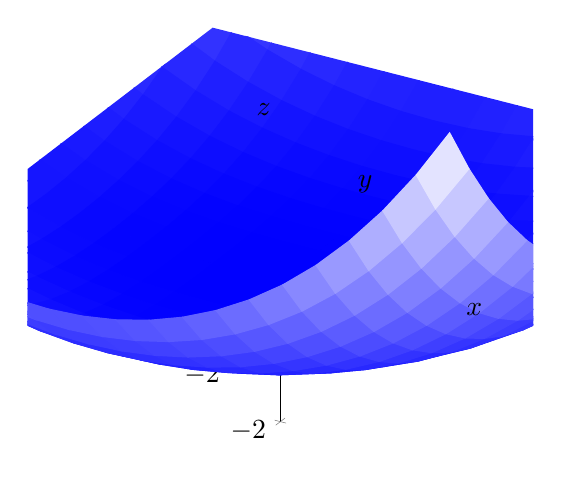
\begin{tikzpicture}
    \begin{axis}[
        axis lines=middle,
        width=8cm, height=8cm,
        view={30}{30}, % 3D view angle
        xmin=-2, xmax=2,
        ymin=-2, ymax=2,
        zmin=-2, zmax=2,
        x label style={at={(ticklabel* cs:1.05)}, anchor=south west},
        y label style={at={(ticklabel* cs:1.05)}, anchor=south east},
        z label style={at={(ticklabel* cs:1.05)}, anchor=south east},
        xlabel={$x$}, ylabel={$y$}, zlabel={$z$}
    ]
    % Draw the orbital surface
    \addplot3[
        surf,
        shader=flat,
        colormap={bluewhite}{color=(blue) color=(white)} % or use a gradient
    ] 
    {sin(sqrt(x^2 + y^2)) * (x^2 + y^2 - 1)}; % Example function, adjust as needed
    \end{axis}
\end{tikzpicture}